\input{header}

\title{Figures, Tables, and Presentation Prep}
\subtitle{ECON 692 -- Applied Economics Seminar}
\author{Andrew Hobbs}
\institute{University of San Francisco}
\date{April 16, 2026}

\begin{document}

\begin{frame}[plain]
  \titlepage
\end{frame}

% ══════════════════════════════════════════════════════════
%  Agenda & Check-in
% ══════════════════════════════════════════════════════════

\begin{frame}{Today's Agenda}
  \small
  \begin{tabular}{@{}r@{\hspace{8pt}}l@{\hspace{16pt}}l@{}}
    \toprule
    \textbf{Time} & \textbf{Duration} & \textbf{Activity} \\
    \midrule
    4:35 & 10 min & Check-in: where are you on the draft? \\
    4:45 & 25 min & What makes a good figure (and table) \\
    5:10 & 10 min & Break \\
    5:20 & 20 min & Group brainstorm: key figures for each project \\
    5:40 & 60 min & Solo work sprint: build your figures \\
    6:40 & 25 min & Reconvene: share figures, get feedback \\
    7:05 & 15 min & Presentation prep: slide design \\
    7:20 & 25 min & Work sprint 2 \\
    7:45 & 10 min & Wrap-up \& next steps \\
    \bottomrule
  \end{tabular}
\end{frame}

\begin{frame}{Check-in}
  \textbf{\textcolor{usfgreen}{Full Draft is due April 24}} --- one week from today.

  \vspace{8pt}

  Quick poll:

  \vspace{4pt}

  \begin{itemize}
    \item Who has at least one polished figure?
    \item Who has a regression table?
    \item Who has started building presentation slides?
  \end{itemize}

  \vspace{8pt}

  Today's goal: leave with your key figures drafted and a plan for your presentation.
\end{frame}

% ══════════════════════════════════════════════════════════
\section{What Makes a Good Figure}
% ══════════════════════════════════════════════════════════

\begin{frame}{What Figures Does Your Project Need?}
  \small
  The answer depends on your method:

  \vspace{6pt}

  \begin{columns}[T]
    \begin{column}{0.48\textwidth}
      \textbf{\textcolor{usfgreen}{DiD / Event Study}}
      \begin{itemize}\setlength\itemsep{0pt}
        \item Event study plot (the money figure)
        \item Pre-trends test
        \item Raw outcome trends by group
      \end{itemize}

      \vspace{4pt}

      \textbf{\textcolor{usfgreen}{Synthetic Control / SDID}}
      \begin{itemize}\setlength\itemsep{0pt}
        \item Treated vs.\ synthetic outcome
        \item Gap plot (treatment effect over time)
        \item Placebo tests
      \end{itemize}
    \end{column}
    \begin{column}{0.48\textwidth}
      \textbf{\textcolor{usfgreen}{IV}}
      \begin{itemize}\setlength\itemsep{0pt}
        \item First-stage scatter / binned scatter
        \item Reduced-form relationship
      \end{itemize}

      \vspace{4pt}

      \textbf{\textcolor{usfgreen}{Everyone}}
      \begin{itemize}\setlength\itemsep{0pt}
        \item Descriptive time series or map
        \item Summary statistics table
        \item Distribution of key variables
      \end{itemize}
    \end{column}
  \end{columns}
\end{frame}

\begin{frame}{Anatomy of a Good Figure}
  Every figure needs these elements:

  \vspace{4pt}

  \begin{enumerate}\setlength\itemsep{1pt}
    \item \textbf{Informative title.} Not ``Figure 1'' --- tell the reader the takeaway.

    \item \textbf{Labeled axes with units.} ``Log earnings (\$2020)'' not just ``Y.''

    \item \textbf{Direct labels on lines.} Almost always better than a legend box.

    \item \textbf{Source note.} Where the data come from, sample size, filters applied.

    \item \textbf{Confidence intervals.} If you're plotting estimates, show uncertainty.
  \end{enumerate}

  \vspace{4pt}

  A figure should be interpretable without reading the surrounding text.
\end{frame}

\begin{frame}{Design Principles: Declutter and Annotate}
  \footnotesize
  \begin{columns}[T]
    \begin{column}{0.48\textwidth}
      \textbf{\textcolor{usfgreen}{Declutter}}
      \begin{itemize}\setlength\itemsep{0pt}
        \item Remove gridlines (or make them very light)
        \item Drop the border/box around the plot
        \item No 3D effects, ever
        \item Maximize the ``data-ink ratio''
      \end{itemize}
    \end{column}
    \begin{column}{0.48\textwidth}
      \textbf{\textcolor{usfgreen}{Annotate}}
      \begin{itemize}\setlength\itemsep{0pt}
        \item Mark key events directly on the plot
        \item Label lines directly instead of using a legend
        \item Add reference lines (zero effect, mean, threshold)
      \end{itemize}
    \end{column}
  \end{columns}

  \vspace{8pt}

  \begin{columns}[T]
    \begin{column}{0.48\textwidth}
      \textbf{\textcolor{usfgreen}{Color with Purpose}}
      \begin{itemize}\setlength\itemsep{0pt}
        \item Use color to distinguish, not decorate
        \item Check colorblind accessibility (viridis, okabe-ito)
        \item Gray out everything that isn't the main message
      \end{itemize}
    \end{column}
    \begin{column}{0.48\textwidth}
      \textbf{\textcolor{usfgreen}{One Message Per Figure}}
      \begin{itemize}\setlength\itemsep{0pt}
        \item If you're showing two things, make two figures
        \item The reader should get the point in 5 seconds
      \end{itemize}
    \end{column}
  \end{columns}
\end{frame}

\begin{frame}{Common Figure Mistakes}
  \small
  \begin{itemize}\setlength\itemsep{1pt}
    \item \textbf{Chartjunk.} Unnecessary gridlines, borders, backgrounds, 3D effects. Strip it all out.

    \item \textbf{Unlabeled or cryptic axes.} ``var\_emp\_q3\_adj'' is not a label. Write ``Employment (thousands).''

    \item \textbf{Too many series.} Eight lines on one plot? Highlight 1--2 and gray out the rest.

    \item \textbf{Misleading scales.} Truncated y-axes, dual axes, inconsistent scales across panels.

    \item \textbf{Default everything.} R and Python defaults are a starting point, not a final product.

    \item \textbf{No annotation of key events.} Policy change at time $t$? Draw a vertical line and label it.
  \end{itemize}
\end{frame}

\begin{frame}{Before: The Cluttered Chart}
  \centering
  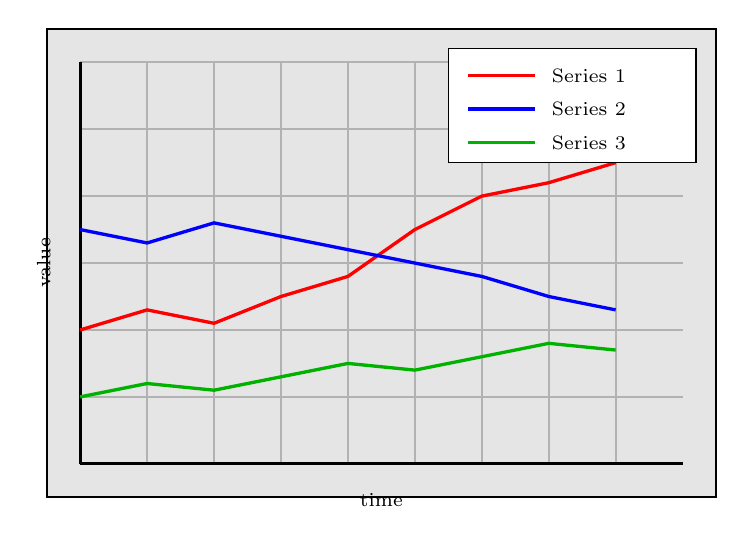
\begin{tikzpicture}[scale=0.85]
    % Gray background
    \fill[gray!20] (-0.5,-0.5) rectangle (9.5,6.5);
    % Border
    \draw[thick, black] (-0.5,-0.5) rectangle (9.5,6.5);
    % Heavy gridlines
    \foreach \y in {1,2,3,4,5,6} {
      \draw[gray!60, thick] (0,\y) -- (9,\y);
    }
    \foreach \x in {1,2,...,8} {
      \draw[gray!60, thick] (\x,0) -- (\x,6);
    }
    % Axes (thick)
    \draw[very thick, black] (0,0) -- (9,0);
    \draw[very thick, black] (0,0) -- (0,6);
    % Y-axis label (unhelpful)
    \node[rotate=90, anchor=south] at (-0.3,3) {\scriptsize value};
    % X-axis label (unhelpful)
    \node[anchor=north] at (4.5,-0.3) {\scriptsize time};
    % Rainbow lines (3 series, garish colors)
    \draw[red, very thick] (0,2) -- (1,2.3) -- (2,2.1) -- (3,2.5) -- (4,2.8) -- (5,3.5) -- (6,4.0) -- (7,4.2) -- (8,4.5);
    \draw[blue, very thick] (0,3.5) -- (1,3.3) -- (2,3.6) -- (3,3.4) -- (4,3.2) -- (5,3.0) -- (6,2.8) -- (7,2.5) -- (8,2.3);
    \draw[green!70!black, very thick] (0,1.0) -- (1,1.2) -- (2,1.1) -- (3,1.3) -- (4,1.5) -- (5,1.4) -- (6,1.6) -- (7,1.8) -- (8,1.7);
    % Legend box (obstructing data)
    \fill[white, draw=black] (5.5,4.5) rectangle (9.2,6.2);
    \draw[red, very thick] (5.8,5.8) -- (6.8,5.8); \node[right, font=\scriptsize] at (6.9,5.8) {Series 1};
    \draw[blue, very thick] (5.8,5.3) -- (6.8,5.3); \node[right, font=\scriptsize] at (6.9,5.3) {Series 2};
    \draw[green!70!black, very thick] (5.8,4.8) -- (6.8,4.8); \node[right, font=\scriptsize] at (6.9,4.8) {Series 3};
  \end{tikzpicture}

  \vspace{2pt}
  {\scriptsize Gray background, heavy gridlines, rainbow colors, useless labels, legend box covering data.}
\end{frame}

\begin{frame}{After: The Clean Chart}
  \centering
  {\footnotesize\textbf{Teen employment fell sharply after the 2020 minimum wage increase}}

  \vspace{2pt}

  \begin{tikzpicture}[scale=0.85]
    % Minimal axes only
    \draw[->, thick] (0,0) -- (9.2,0);
    \draw[->, thick] (0,0) -- (0,6.2);
    % Light reference gridlines (horizontal only)
    \foreach \y in {2,4} {
      \draw[gray!25] (0,\y) -- (9,\y);
    }
    % Y-axis ticks and labels
    \foreach \y/\lab in {0/0, 2/200, 4/400, 6/600} {
      \draw (0,\y) -- (-0.1,\y) node[left, font=\scriptsize] {\lab};
    }
    % X-axis ticks and labels
    \foreach \x/\lab in {0/2016, 2/2018, 4/2020, 6/2022, 8/2024} {
      \draw (\x,0) -- (\x,-0.1) node[below, font=\scriptsize] {\lab};
    }
    % Axis labels
    \node[rotate=90, anchor=south, font=\scriptsize] at (-0.7,3) {Employment (thousands)};
    % Policy line
    \draw[dashed, gray!50] (4,0) -- (4,5.5);
    \node[font=\scriptsize, gray!70!black, anchor=south] at (4,5.5) {MW increase};
    % Treatment line (bold, green)
    \draw[usfgreen, line width=1.5pt] (0,2) -- (1,2.3) -- (2,2.1) -- (3,2.5) -- (4,2.8) -- (5,3.5) -- (6,4.0) -- (7,4.2) -- (8,4.5);
    % Control line (gray)
    \draw[gray!60, thick] (0,3.5) -- (1,3.3) -- (2,3.6) -- (3,3.4) -- (4,3.2) -- (5,3.0) -- (6,2.8) -- (7,2.5) -- (8,2.3);
    % Direct labels
    \node[right, font=\scriptsize, usfgreen] at (8.1,4.5) {Treated};
    \node[right, font=\scriptsize, gray!60] at (8.1,2.3) {Control};
    % Annotation arrow for gap
    \draw[<->, thick, usfgold] (7,2.5) -- (7,4.2);
    \node[right, font=\scriptsize, usfgold!80!black] at (7.1,3.35) {Gap};
    % Source note
    \node[anchor=north west, font=\tiny, gray] at (0,-0.8) {Source: CPS monthly data, ages 16--19. $N = 48{,}000$.};
  \end{tikzpicture}
\end{frame}

\begin{frame}{What Changed?}
  \begin{columns}[T]
    \begin{column}{0.48\textwidth}
      \textbf{\textcolor{red!60}{Before}}
      \begin{itemize}\setlength\itemsep{1pt}
        \item Gray background, thick gridlines
        \item Legend box covering data
        \item Axis labels: ``value'' and ``time''
        \item Rainbow color palette
        \item No title, no source note
        \item Three unnamed ``series''
      \end{itemize}
    \end{column}
    \begin{column}{0.48\textwidth}
      \textbf{\textcolor{usfgreen}{After}}
      \begin{itemize}\setlength\itemsep{1pt}
        \item White background, minimal gridlines
        \item Direct labels on lines
        \item ``Employment (thousands)''
        \item Two purposeful colors + annotation
        \item Title states the finding
        \item Source note with sample info
      \end{itemize}
    \end{column}
  \end{columns}

  \vspace{8pt}

  The data are identical. The difference is \textbf{design}. Use \texttt{theme\_minimal()} as a starting point, then customize from there.
\end{frame}

\begin{frame}{Misleading: The Truncated Y-Axis}
  \small
  A 3-percentage-point difference made to look enormous.

  \vspace{4pt}

  \begin{columns}[T]
    \begin{column}{0.48\textwidth}
      \centering
      \textbf{\textcolor{red!60}{Misleading}}

      \vspace{2pt}

      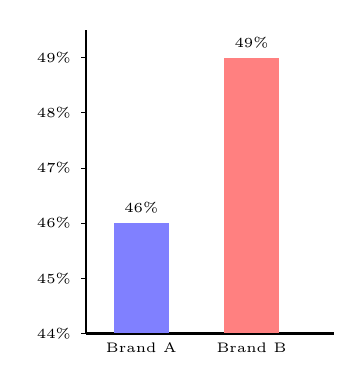
\begin{tikzpicture}[scale=0.7]
        % Axes
        \draw[thick] (0,0) -- (4.5,0);
        \draw[thick] (0,0) -- (0,5.5);
        % Y-axis starts at 44% — truncated!
        \foreach \y/\lab in {0/44, 1/45, 2/46, 3/47, 4/48, 5/49} {
          \draw (0,\y) -- (-0.1,\y) node[left, font=\tiny] {\lab\%};
        }
        % Bars
        \fill[blue!50] (0.5,0) rectangle (1.5,2);  % 46%
        \fill[red!50] (2.5,0) rectangle (3.5,5);   % 49%
        % Labels
        \node[font=\tiny, below] at (1,0) {Brand A};
        \node[font=\tiny, below] at (3,0) {Brand B};
        \node[font=\tiny, above] at (1,2) {46\%};
        \node[font=\tiny, above] at (3,5) {49\%};
      \end{tikzpicture}

      {\scriptsize Brand B looks 2.5$\times$ taller!}
    \end{column}
    \begin{column}{0.48\textwidth}
      \centering
      \textbf{\textcolor{usfgreen}{Honest}}

      \vspace{2pt}

      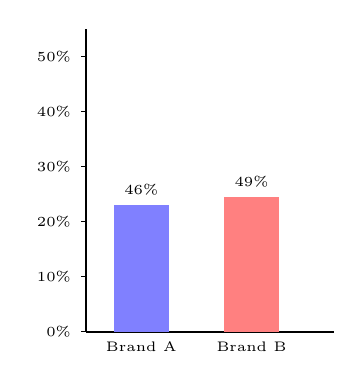
\begin{tikzpicture}[scale=0.7]
        % Axes
        \draw[thick] (0,0) -- (4.5,0);
        \draw[thick] (0,0) -- (0,5.5);
        % Y-axis starts at 0%
        \foreach \y/\lab in {0/0, 1/10, 2/20, 3/30, 4/40, 5/50} {
          \draw (0,\y) -- (-0.1,\y) node[left, font=\tiny] {\lab\%};
        }
        % Bars — now proportional
        \fill[blue!50] (0.5,0) rectangle (1.5,2.3);  % 46%
        \fill[red!50] (2.5,0) rectangle (3.5,2.45);  % 49%
        % Labels
        \node[font=\tiny, below] at (1,0) {Brand A};
        \node[font=\tiny, below] at (3,0) {Brand B};
        \node[font=\tiny, above] at (1,2.3) {46\%};
        \node[font=\tiny, above] at (3,2.45) {49\%};
      \end{tikzpicture}

      {\scriptsize The real difference: 3 points.}
    \end{column}
  \end{columns}

  \vspace{6pt}

  Tufte called this the \textbf{``lie factor''}: the ratio of the visual effect to the data effect. If the axis doesn't start at zero for a bar chart, ask why.
\end{frame}

\begin{frame}{Misleading: The Inverted Axis}
  \small
  Inspired by a real Reuters graphic on Florida gun deaths.

  \vspace{2pt}

  \begin{columns}[T]
    \begin{column}{0.48\textwidth}
      \centering
      \textbf{\textcolor{red!60}{Misleading}}

      \vspace{2pt}

      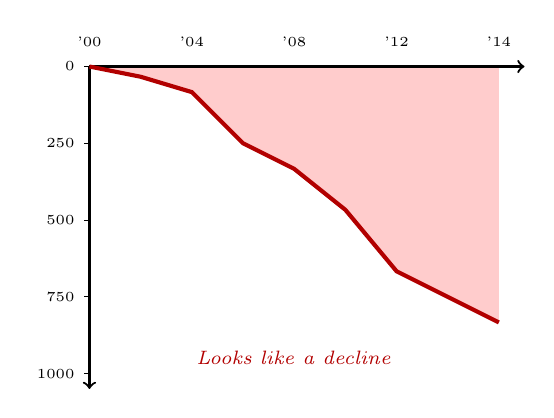
\begin{tikzpicture}[scale=0.65]
        % Red background fill under curve (inverted)
        \fill[red!20] (0,6) -- (1,5.8) -- (2,5.5) -- (3,4.5) -- (4,4.0)
          -- (5,3.2) -- (6,2.0) -- (7,1.5) -- (8,1.0)
          -- (8,6) -- cycle;
        % Axes — y-axis is inverted (high values at bottom)
        \draw[->, thick] (0,6) -- (0,-0.3);
        \draw[->, thick] (0,6) -- (8.5,6);
        % Y-axis labels (inverted: 0 at top, 1000 at bottom)
        \foreach \y/\lab in {6/0, 4.5/250, 3/500, 1.5/750, 0/1000} {
          \draw (0,\y) -- (-0.1,\y) node[left, font=\tiny] {\lab};
        }
        % X-axis labels
        \foreach \x/\lab in {0/'00, 2/'04, 4/'08, 6/'12, 8/'14} {
          \node[font=\tiny, above] at (\x,6.2) {\lab};
        }
        % The line
        \draw[red!70!black, line width=1.5pt] (0,6) -- (1,5.8) -- (2,5.5) -- (3,4.5)
          -- (4,4.0) -- (5,3.2) -- (6,2.0) -- (7,1.5) -- (8,1.0);
        % Looks like deaths are falling
        \node[font=\scriptsize, red!70!black] at (4,0.3) {\textit{Looks like a decline}};
      \end{tikzpicture}
    \end{column}
    \begin{column}{0.48\textwidth}
      \centering
      \textbf{\textcolor{usfgreen}{Corrected}}

      \vspace{2pt}

      \begin{tikzpicture}[scale=0.65]
        % Axes — standard orientation
        \draw[->, thick] (0,0) -- (8.5,0);
        \draw[->, thick] (0,0) -- (0,6.5);
        % Y-axis labels (standard)
        \foreach \y/\lab in {0/0, 1.5/250, 3/500, 4.5/750, 6/1000} {
          \draw (0,\y) -- (-0.1,\y) node[left, font=\tiny] {\lab};
        }
        % X-axis labels
        \foreach \x/\lab in {0/'00, 2/'04, 4/'08, 6/'12, 8/'14} {
          \node[font=\tiny, below] at (\x,-0.1) {\lab};
        }
        % The line — same data, standard orientation
        \draw[usfgreen, line width=1.5pt] (0,0) -- (1,0.2) -- (2,0.5) -- (3,1.5)
          -- (4,2.0) -- (5,2.8) -- (6,4.0) -- (7,4.5) -- (8,5.0);
        % Now it's obvious: deaths are rising
        \node[font=\scriptsize, usfgreen!70!black] at (4,5.7) {\textit{Deaths nearly doubled}};
      \end{tikzpicture}
    \end{column}
  \end{columns}

  \vspace{4pt}

  Same data. Flipping the y-axis made a \textbf{dramatic increase} look like a decline. Always check axis orientation.
\end{frame}

\begin{frame}{The Data-Ink Ratio}
  \small
  Tufte's principle: maximize the share of ink that shows \textbf{data}. Erase everything else.

  \vspace{4pt}

  \begin{columns}[T]
    \begin{column}{0.32\textwidth}
      \centering
      \textbf{Step 1: Default}

      \vspace{2pt}

      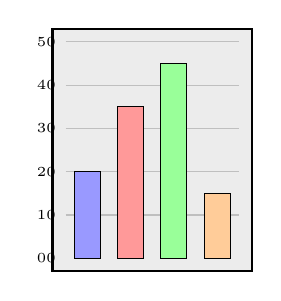
\begin{tikzpicture}[scale=0.55]
        % Full frame box
        \fill[gray!15] (-0.3,-0.3) rectangle (4.3,5.3);
        \draw[thick] (-0.3,-0.3) rectangle (4.3,5.3);
        % Gridlines
        \foreach \y in {1,2,3,4,5} {
          \draw[gray!50] (0,\y) -- (4,\y);
        }
        % Bars with borders and pattern
        \fill[blue!40, draw=black] (0.2,0) rectangle (0.8,2);
        \fill[red!40, draw=black] (1.2,0) rectangle (1.8,3.5);
        \fill[green!40, draw=black] (2.2,0) rectangle (2.8,4.5);
        \fill[orange!40, draw=black] (3.2,0) rectangle (3.8,1.5);
        % Y-axis
        \foreach \y in {0,1,...,5} {
          \node[left, font=\tiny] at (0,\y) {\y0};
        }
      \end{tikzpicture}

      {\tiny Background, borders,\\ gridlines, 4 colors}
    \end{column}
    \begin{column}{0.32\textwidth}
      \centering
      \textbf{Step 2: Remove}

      \vspace{2pt}

      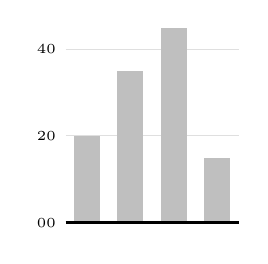
\begin{tikzpicture}[scale=0.55]
        % No background, no frame
        % Light gridlines only
        \foreach \y in {2,4} {
          \draw[gray!25] (0,\y) -- (4,\y);
        }
        % Bars — single color, no border
        \fill[gray!50] (0.2,0) rectangle (0.8,2);
        \fill[gray!50] (1.2,0) rectangle (1.8,3.5);
        \fill[gray!50] (2.2,0) rectangle (2.8,4.5);
        \fill[gray!50] (3.2,0) rectangle (3.8,1.5);
        % Minimal axis
        \draw[thick] (0,0) -- (4,0);
        \foreach \y in {0,2,4} {
          \node[left, font=\tiny] at (0,\y) {\y0};
        }
      \end{tikzpicture}

      {\tiny White background,\\ fewer gridlines, one color}
    \end{column}
    \begin{column}{0.32\textwidth}
      \centering
      \textbf{Step 3: Label}

      \vspace{2pt}

      \begin{tikzpicture}[scale=0.55]
        % No gridlines at all
        % Bars — highlight the key one
        \fill[gray!35] (0.2,0) rectangle (0.8,2);
        \fill[gray!35] (1.2,0) rectangle (1.8,3.5);
        \fill[usfgreen!60] (2.2,0) rectangle (2.8,4.5);
        \fill[gray!35] (3.2,0) rectangle (3.8,1.5);
        % Direct labels
        \node[above, font=\tiny] at (0.5,2) {20};
        \node[above, font=\tiny] at (1.5,3.5) {35};
        \node[above, font=\tiny, usfgreen!80!black] at (2.5,4.5) {\textbf{45}};
        \node[above, font=\tiny] at (3.5,1.5) {15};
        % Category labels
        \node[below, font=\tiny] at (0.5,0) {Q1};
        \node[below, font=\tiny] at (1.5,0) {Q2};
        \node[below, font=\tiny, usfgreen!80!black] at (2.5,0) {\textbf{Q3}};
        \node[below, font=\tiny] at (3.5,0) {Q4};
        % Baseline only
        \draw[thick] (0,0) -- (4,0);
      \end{tikzpicture}

      {\tiny Direct labels, highlight\\ the message, no gridlines}
    \end{column}
  \end{columns}

  \vspace{6pt}

  \textbf{Data-ink ratio} $=$ \textrm{data ink} $/$ \textrm{total ink}. Each step removes non-data ink without losing information.
\end{frame}

% ══════════════════════════════════════════════════════════
\section{Tables}
% ══════════════════════════════════════════════════════════

\begin{frame}{Regression Table Essentials}
  \footnotesize
  A good regression table has:

  \vspace{2pt}

  \begin{columns}[T]
    \begin{column}{0.48\textwidth}
      \begin{enumerate}\setlength\itemsep{1pt}
        \item \textbf{Clear column headers.} Each column = one specification. Label what changes: ``+ Controls,'' ``+ FE,'' ``Alt.\ Sample.''
        \item \textbf{Readable variable names.} Not \texttt{log\_inc\_cpi\_adj}. Write ``Log income (2020 \$).''
        \item \textbf{Standard errors.} In parentheses, with a note on clustering level.
        \item \textbf{Stars --- but don't overdo it.} One system (*$p<0.05$), applied consistently.
      \end{enumerate}
    \end{column}
    \begin{column}{0.48\textwidth}
      \begin{enumerate}\setlength\itemsep{1pt}
        \setcounter{enumi}{4}
        \item \textbf{N, $R^2$, FE indicators.} At the bottom. Use Yes/No rows for fixed effects.
        \item \textbf{Only show key coefficients.} Don't report every control. The reader cares about your treatment effect.
        \item \textbf{Notes.} Clustering, sample restrictions, variable definitions.
      \end{enumerate}

      \vspace{2pt}

      {\scriptsize Tools: \texttt{etable()} in \texttt{fixest}, \texttt{modelsummary()}, \texttt{stargazer()}.}
    \end{column}
  \end{columns}
\end{frame}

% ══════════════════════════════════════════════════════════
\section{Group Brainstorm}
% ══════════════════════════════════════════════════════════

\begin{frame}{Activity: Figure Brainstorm}
  \textbf{Form groups of 3--4.}

  \vspace{8pt}

  \textbf{Round 1} (2 min each): Briefly describe your project --- question, method, data.

  \vspace{4pt}

  \textbf{Round 2} (5 min each): As a group, brainstorm the key figures for each person's project. For each figure, write down:
  \begin{itemize}
    \item What it shows (one sentence)
    \item What goes on each axis
    \item Why it matters for the argument
  \end{itemize}

  \vspace{8pt}

  Aim for \textbf{3--5 figures per project}. You don't need all of them --- but you need to know which ones matter most.
\end{frame}

\begin{frame}{Guiding Questions}
  As you brainstorm, ask:

  \vspace{6pt}

  \begin{enumerate}
    \item \textbf{What's the one figure a reader remembers?} The event study, gap plot, or scatter that \emph{is} your result.

    \vspace{3pt}

    \item \textbf{What shows your identification works?} Pre-trends, balance tests, first-stage strength, placebos.

    \vspace{3pt}

    \item \textbf{What descriptive fact motivates the question?} A trend, a map, a distribution.

    \vspace{3pt}

    \item \textbf{What does the skeptic want to see?} Robustness, heterogeneity, alternative specifications.
  \end{enumerate}

  \vspace{6pt}

  Rank your list. Start building from the top.
\end{frame}

% ══════════════════════════════════════════════════════════
\section{Work Sprint}
% ══════════════════════════════════════════════════════════

\begin{frame}{Work Sprint 1 (5:40--6:40)}
  Build your figures. Start with the most important one.

  \vspace{6pt}

  \textbf{Priority order:}
  \begin{enumerate}\setlength\itemsep{1pt}
    \item \textbf{Main result figure.} Event study, SC plot, IV scatter --- whatever shows your key finding.
    \item \textbf{Identification figure.} Pre-trends, balance, first stage --- whatever builds credibility.
    \item \textbf{Descriptive motivation.} The fact or pattern that makes the reader care.
  \end{enumerate}

  \vspace{6pt}

  \textbf{Tips:} Start with the simplest version --- get data on the plot first, then polish. Use \texttt{theme\_minimal()} as your base. Save as PDF or PNG at high resolution.
\end{frame}

% ══════════════════════════════════════════════════════════
\section{Reconvene}
% ══════════════════════════════════════════════════════════

\begin{frame}{Reconvene: Share Your Figures (6:40--7:05)}
  Back in your groups. Each person: show 1--2 figures.

  \vspace{8pt}

  \textbf{Feedback protocol:}

  \vspace{4pt}

  \begin{enumerate}
    \item \textbf{First impression.} Look at the figure for 10 seconds without explanation. What do you think it shows?

    \vspace{2pt}

    \item \textbf{Clarity check.} Can you read the axes? Do you know the units? Is the takeaway obvious?

    \vspace{2pt}

    \item \textbf{What's missing?} Labels, annotations, confidence intervals, reference lines, title?

    \vspace{2pt}

    \item \textbf{Does it support the argument?} Is this the right figure for the point being made?
  \end{enumerate}

  \vspace{8pt}

  If your group can't tell what the figure shows without your explanation, that's the most useful feedback you'll get.
\end{frame}

% ══════════════════════════════════════════════════════════
\section{Presentation Prep}
% ══════════════════════════════════════════════════════════

\begin{frame}{Final Presentations: The Setup}
  \begin{itemize}
    \item \textbf{May 7:} First group ($\sim$3 presenters, 1 hour)
    \item \textbf{May 14:} Remaining presenters (full class period)
    \item \textbf{About 15 minutes each} including Q\&A
  \end{itemize}

  \vspace{8pt}

  Target: \textbf{$\sim$12--15 slides} for 12--13 minutes of talking, plus 2--3 minutes for questions.

  \vspace{8pt}

  We'll finalize the schedule and order next week.
\end{frame}

\begin{frame}{Pick Your Date}
  \begin{columns}[c]
    \begin{column}{0.55\textwidth}
      Please fill out the survey so we can set the schedule:

      \vspace{8pt}

      \begin{itemize}
        \item \textbf{May 7:} $\sim$3 slots (first hour of class)
        \item \textbf{May 14:} $\sim$10 slots (full period)
        \item Either date works? Say so --- it helps with scheduling.
      \end{itemize}

      \vspace{8pt}

      {\small\texttt{tinyurl.com} --- or just scan the QR code $\to$}
    \end{column}
    \begin{column}{0.4\textwidth}
      \centering
      
\includegraphics[width=0.85\textwidth]{../Figures/presentation_survey_qr.png}

      \vspace{4pt}

      {\footnotesize Presentation Date Survey}
    \end{column}
  \end{columns}
\end{frame}

\begin{frame}{Slide Design Principles}
  \begin{enumerate}
    \item \textbf{One idea per slide.} If you need two bullet lists, make two slides.

    \vspace{3pt}

    \item \textbf{Assertion--evidence structure.} The slide title is your claim: ``Minimum wage increases reduced teen employment by 3\%.'' The body is the evidence: the figure or table that proves it.

    \vspace{3pt}

    \item \textbf{More figures, less text.} Your slides aren't a script. Use them to show evidence; you provide the narration.

    \vspace{3pt}

    \item \textbf{Big fonts, big figures.} If someone in the back row can't read it, make it bigger.

    \vspace{3pt}

    \item \textbf{Build the narrative.} Motivation $\to$ question $\to$ data $\to$ method $\to$ results $\to$ so what. Same arc as the project, just compressed.
  \end{enumerate}
\end{frame}

\begin{frame}{Presentation Structure Template}
  \footnotesize
  A 15-minute economics presentation, slide by slide:

  \vspace{2pt}

  \begin{columns}[T]
    \begin{column}{0.48\textwidth}
      \begin{enumerate}\setlength\itemsep{0pt}
        \item Title slide
        \item Motivation (the hook)
        \item Research question
        \item Related work (1 slide max)
        \item Data overview
        \item Summary statistics
        \item Empirical strategy
      \end{enumerate}
    \end{column}
    \begin{column}{0.48\textwidth}
      \begin{enumerate}\setlength\itemsep{0pt}
        \setcounter{enumi}{7}
        \item Identification (why it's credible)
        \item Main result (the money slide)
        \item Robustness / mechanisms
        \item Interpretation \& implications
        \item Conclusion (1 slide)
      \end{enumerate}

      \vspace{2pt}

      That's 12 slides. Spend most of your time on 7--10.
    \end{column}
  \end{columns}

  \vspace{4pt}

  \textbf{Common mistake:} spending 8 minutes on background and 4 on results. Flip that.
\end{frame}

% ══════════════════════════════════════════════════════════
\section{Work Sprint 2}
% ══════════════════════════════════════════════════════════

\begin{frame}{Work Sprint 2 (7:20--7:45)}
  Pick your priority:

  \vspace{8pt}

  \begin{columns}[T]
    \begin{column}{0.48\textwidth}
      \textbf{\textcolor{usfgreen}{Figures Track}}
      \begin{enumerate}
        \item Apply feedback from your group
        \item Polish labels, colors, annotations
        \item Start your second or third figure
      \end{enumerate}
    \end{column}
    \begin{column}{0.48\textwidth}
      \textbf{\textcolor{usfgreen}{Slides Track}}
      \begin{enumerate}
        \item Set up your slide deck (Google Slides, Beamer, Quarto)
        \item Build your title + motivation slides
        \item Drop in existing figures
      \end{enumerate}
    \end{column}
  \end{columns}

  \vspace{10pt}

  Whatever you don't finish today, do before next week.
\end{frame}

% ══════════════════════════════════════════════════════════
\section{Wrap-up}
% ══════════════════════════════════════════════════════════

\begin{frame}{Next Week \& Deadlines}
  \textbf{Next week (4/23):} Peer review workshop and presentation practice.

  \vspace{8pt}

  \textbf{Upcoming:}
  \begin{itemize}
    \item Weekly progress report due \textbf{Wednesday}
    \item \textbf{\textcolor{usfgreen}{Full Draft due April 24}} (one week)
    \item Final presentations: May 7 \& May 14
  \end{itemize}

  \vspace{8pt}

  \begin{block}{Between Now and the Full Draft}
    Your full draft needs: intro, data description, empirical strategy, results with figures and tables, and conclusion. Leave today with your key figures built, and you're in good shape.
  \end{block}
\end{frame}

\end{document}
